\documentclass{beamer}

\mode<presentation>
{
	\usetheme{Madrid}
}

\usepackage{graphics, graphicx}
\usepackage{booktabs}
\usepackage{url}
\DeclareGraphicsExtensions{.pdf,.png,.jpg,.gif}

\title{Linux Beginner Guide}

\author{Jaewoong Lee}

\institute[UNIST]
{
	Ulsan National Institute of Science and Technology
	\medskip
	\newline
	\textit{jwlee230@unist.ac.kr}
}

\date{\today}

\begin{document}
	\begin{frame}
		\titlepage
	\end{frame}

	\begin{frame}
		\frametitle{Introduction}
		
		In this guide, I assume that followings are already installed:
		\begin{enumerate}
			\item Ubuntu 16.04.2 or Higher
			\item ZSH 5.0.2 or Higher
			\item VIM 8.1 or Higher
			\item Python 3
			\item We will connect to server via SSH
		\end{enumerate}
	
		Also, you should be familiar with Linux system. 
		
		If not so, you should start at here: \url{https://github.com/Fumire/LinuxLecture/releases/tag/200105}
	\end{frame}

	\begin{frame}
		\frametitle{Overview}
		\tableofcontents
	\end{frame}

	\section{Python?}
	\begin{frame}
		\frametitle{Python?}
		
		\begin{figure}
			\centering
			
\includegraphics[width=0.2 \linewidth]{figures/python.png}
			\caption{Logo of Python}
		\end{figure}
	
		Python is an \textit{interpreted} programming language, created by Guido van Rossum in 1991. 
	\end{frame}

	\begin{frame}
		\frametitle{Interpreted?}
		
		Interpreted is opposed \textit{compiled}.
		
		Complied programming language is required compiling(translating) before its running. 
		
		Interpreted programming language does not require compiling; it can run by read code one-by-one line. 
	\end{frame}

	\begin{frame}
		\frametitle{How to run Python?}
		There are two ways to run Python
		\begin{figure}
			\centering
			$\begin{array}{cc}
				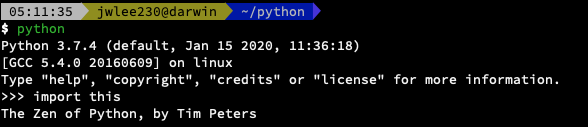
\includegraphics[width=0.4 \linewidth]{figures/run1.png}
				&
				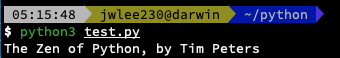
\includegraphics[width=0.4 \linewidth]{figures/run2.png}
				\\
				
				\mbox{(a) Python Interpreter} & \mbox{(b) Python Script} \\
			\end{array}$
		\end{figure}
	
		We will prefer (b) Python Script for better reproducibility. 
	\end{frame}
	
	\section{Basic IO}
	\begin{frame}
		\frametitle{print()}
		\begin{example}
			print("Hello world")
		\end{example}
		This example will print as:
		\begin{example}
			Hello world
		\end{example}
		Try with other strings!
	\end{frame}

	\begin{frame}
		\frametitle{input()}
		\begin{example}
			s = input("Write:") \\
			print(s)
		\end{example}
		input() accepts input as string.
		
		Also, in this example, \textit{variable} is used; we will talk about that later. 
	\end{frame}
	
	\section{Data Types}
	\begin{frame}
		\frametitle{int Type}
		\textit{int} type means integer. You can obviously use integers in Python.
		\begin{example}
			print(123) \\
			print(-321) \\
			print(0)
		\end{example}
		Also, you can use octal and hexadecimal integers as:
		\begin{example}
			print(0o123) \\
			print(0xABC)
		\end{example}
	\end{frame}

	\begin{frame}
		\frametitle{float Type}
		\textit{float} type means decimals.
		\begin{example}
			print(1.23) \\
			print(-.3.21)
		\end{example}
		Also, you can express decimals as:
		\begin{example}
			print(1.23e45) \\
			print(6.78E-9)
		\end{example}
		Those mean $1.23 \times 10^{45}$ and $6.78 \times 10^{-9}$, respectively.
	\end{frame}

	\begin{frame}
		\frametitle{Arithmetic Operators}
		You might know how to express arithmetic operators in programming.
		\begin{example}
			print(3 + 4) \\
			print(3 - 4) \\
			print(3 * 4) \\
			print(3 / 4) 
		\end{example}
	
		is equivalent with
		
		\begin{example}
			3 + 4 \\
			3 - 4 \\
			3 $\times$ 4 \\
			3 $\div$ 4
		\end{example}
	\end{frame}

	\begin{frame}
		\frametitle{Power Operator}
		There is power operator in Python.
		\begin{example}
			print(3 ** 4)
		\end{example}
		will return as
		\begin{example}
			$3^4$ = 81
		\end{example}
	\end{frame}

	\begin{frame}
		\frametitle{Remainder Operator}
		The '\%' operator results remainder.
		
		\begin{example}
			print(15 \% 4)
		\end{example}
	
		The example will print '3'.
	\end{frame}

	\begin{frame}
		\frametitle{Quotient Operator}
		The '//' opertor results quotient.
		
		\begin{example}
			print(15 / 4)
			print(15 // 4)
		\end{example}
	
		Compare the difference of above example. 
	\end{frame}

		
	\section{Advanced IO}
	
	\section{IF, FOR, and WHILE}

	\section{Funtion}
	
	\section{Handling Exception}
	
	\section{Module}
\end{document}